Für eine eventuelle BIAS-Korrektur kommt eine bisherige Herangehensweise nicht in Frage, da dadurch die lokale und vor allem zeitliche Varianz zu stark beeinträchtigt wird wie in Abb. \ref{fig:boxplot_corrected_rcp} zu erkennen ist. Laut D.Maraun \cite{biasMaraun} ist dafür ein Herangehensweise über stochastische Quantile-Mapping nötig. Dabei ist vor allem auf Überkorrektur acht zu geben, welche sich durch die Überschätzung der Flächenmittelwerte für Extremniederschläge und falsche Trends äußert. Die von Maraun in \cite{biasMaraun} postulierte Herangehensweise wird in diesem Kapitel verfolgt.
\section{Herangehensweise}
\begin{itemize}
	\item Zunächst wurden die am stärksten von Abweichungen betroffenen Regionen ausgemacht. Dies erfolgte über die Jahreszeiten bzw. Monate.
\end{itemize}

\section{Am stärksten betroffen Regionen}
Die betreffenden Datensätze (historical, evaluation und APGD) wurden zunächst in monatliche Abschnitte unterteilt. Diese wurden dann einer Quantil-Berechnung über alle Jahre unterzogen. In Folge wurden die 20 größten und 20 kleinsten Abweichungen von den entsprechenden Quantilen des Beobachtungsdatensatzes den Monaten entsprechend auf einer Karte abgebildet um die am stärksten betroffenen Regionen zu erkennen. Die Ergebnisse sind in Abb. \ref{fig:decision_plot_q90-hist}-\ref{fig:decision_plot_q99-eval} zu erkennen, Die in Rechtecken gekennzeichneten Regionen werden in Folge nach Jahreszeiten näher betrachtet, da in ihnen die größten Abweichungen herrschen. Die Regionen, die als ''mixed'' gekennzeichnet sind haben eine zu große Fluktuation über die Jahreszeiten um sie einer gewissen Jahreszeit zuordnen zu können. Man erkennt im Vergleich der unterschiedlichen Datensätze, dass die Abweichung in gewissen Regionen konstant bleibt. Sie befinden sich ungefähr auf derselben Position über alle Datensätze und auch größtenteils über die unterschiedlichen Quantile, was für die folgenden Berechnungen von Vorteil ist. Wie man in Abb.\ref{fig:decision_plot_q99-eval} erkennen kann befindet sich in der südöstlichen Region (um die Stadt Split) eine Zone, die extreme Abweichungen im 99.Quantil über alle Monate zeigt, dies deutet sich bereits in der Abbildung des 90. Quantils ab (Abb. \ref{fig:decision_plot_q90-eval}). Um die Darstellung zu verbessern und die Ausreißer zu minimieren wird diese Region zunächst aus den folgenden Berechnungen ausgeschnitten und außen vor gelassen. 


\begin{figure}[h!]
	\centering{
	\begin{subfigure}{0.49\textwidth}
		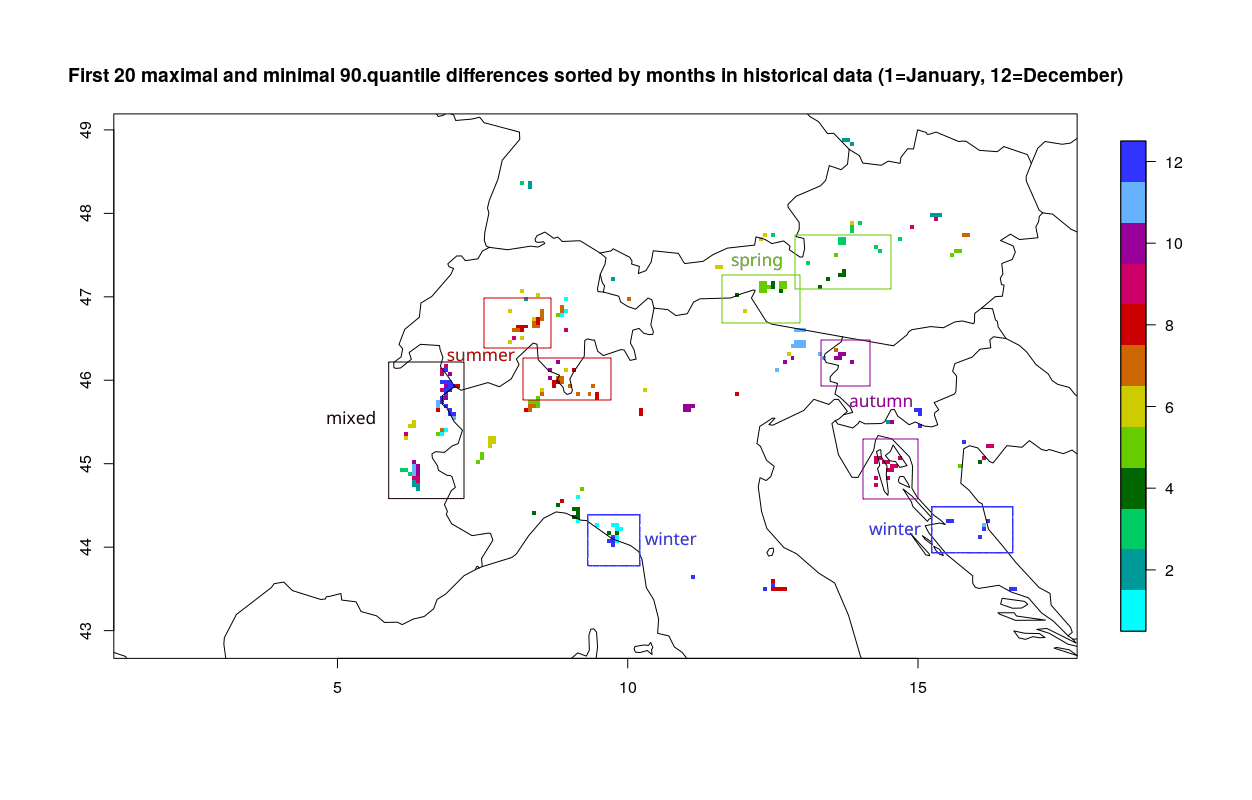
\includegraphics[angle=270, width=\textwidth]{/quantile/decision_plot_q90-hist.png}
		\caption{Die 40 größten Abweichungen im 90.Quantil des historical-Datensatzes.}
		\label{fig:decision_plot_q90-hist}
	\end{subfigure}
	\begin{subfigure}{0.49\textwidth}
		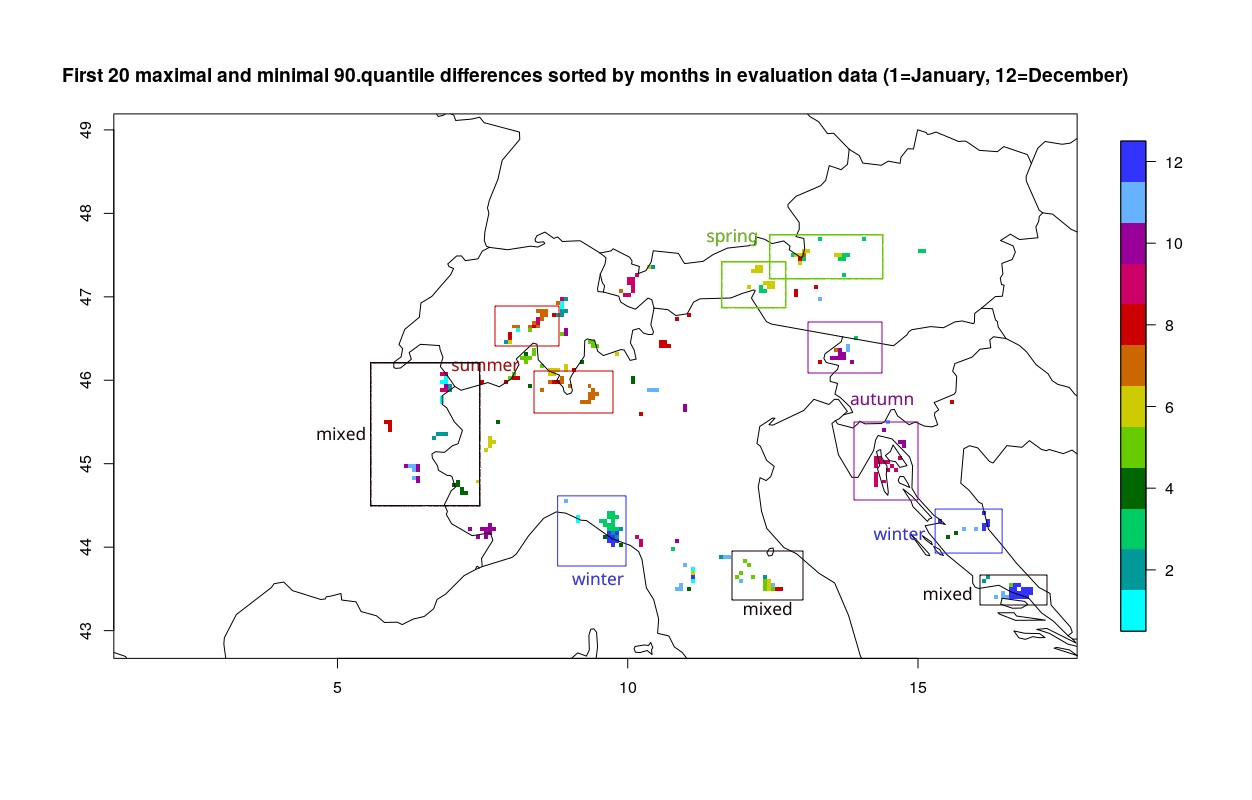
\includegraphics[angle=270, width=\textwidth]{/quantile/decision_plot_q90-eval.png}
		\caption{Die 40 größten Abweichungen im 90.Quantil des evaluation-Datensatzes.}
		\label{fig:decision_plot_q90-eval}
	\end{subfigure}
	\begin{subfigure}{0.49\textwidth}
		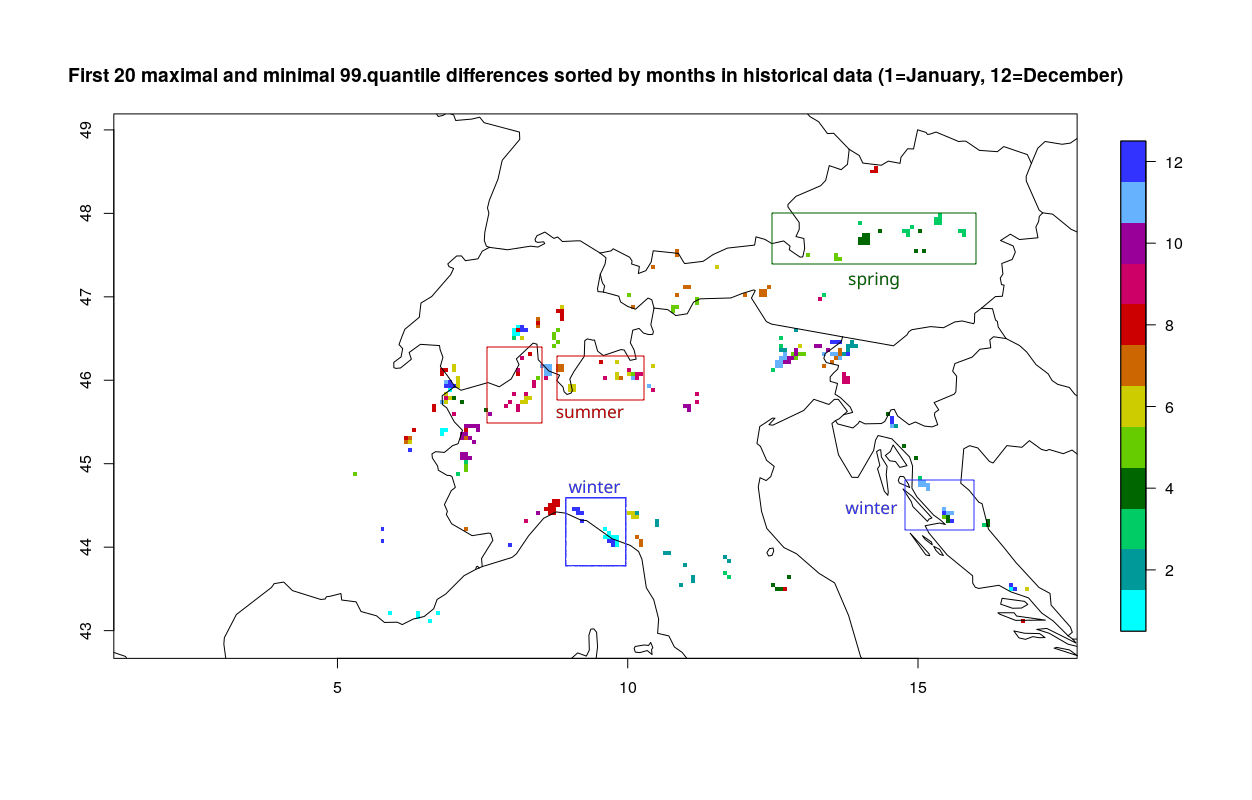
\includegraphics[angle=270, width=\textwidth]{/quantile/decision_plot_q99-hist.png}
		\caption{Die 40 größten Abweichungen im 99.Quantil des historical-Datensatzes.}
		\label{fig:decision_plot_q99-hist}
	\end{subfigure}
	\begin{subfigure}{0.49\textwidth}
		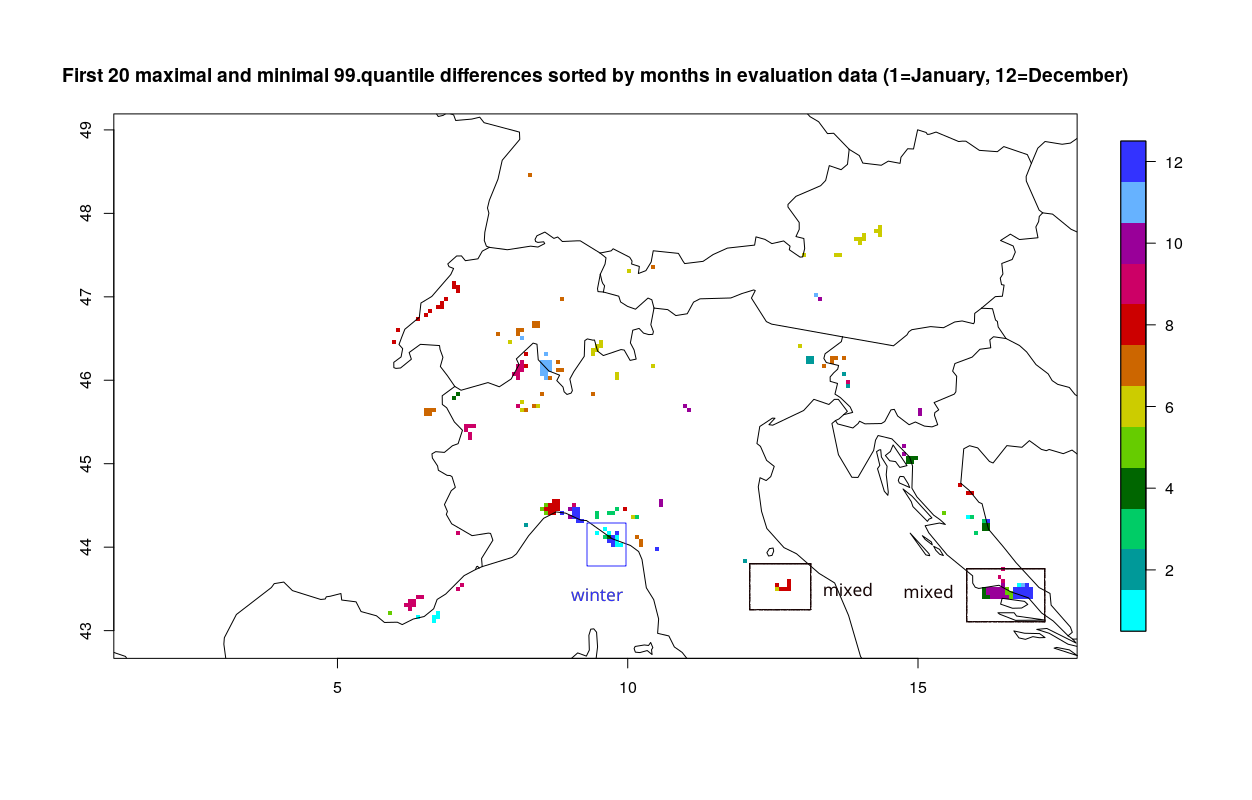
\includegraphics[angle=270,width=\textwidth]{/quantile/decision_plot_q99-eval.png}
		\caption{Die 40 größten Abweichungen im 99.Quantil des evaluation-Datensatzes.}
		\label{fig:decision_plot_q99-eval}
	\end{subfigure}
}
\end{figure}